\section{Import volume protocol}
\label{app:importVolume}%a100
   
 \begin{itemize}
  \item \scipion menu:\\
  \ttt{Protocols SPA -> Imports} (\ffigure{fig:app_protocol_volume_1} (A))\\
  
  \item Protocol form parameters (\ffigure{fig:app_protocol_volume_1} (B)):\\
  
  \begin{figure}[H]
    \centering 
    \captionsetup{width=.7\linewidth} 
    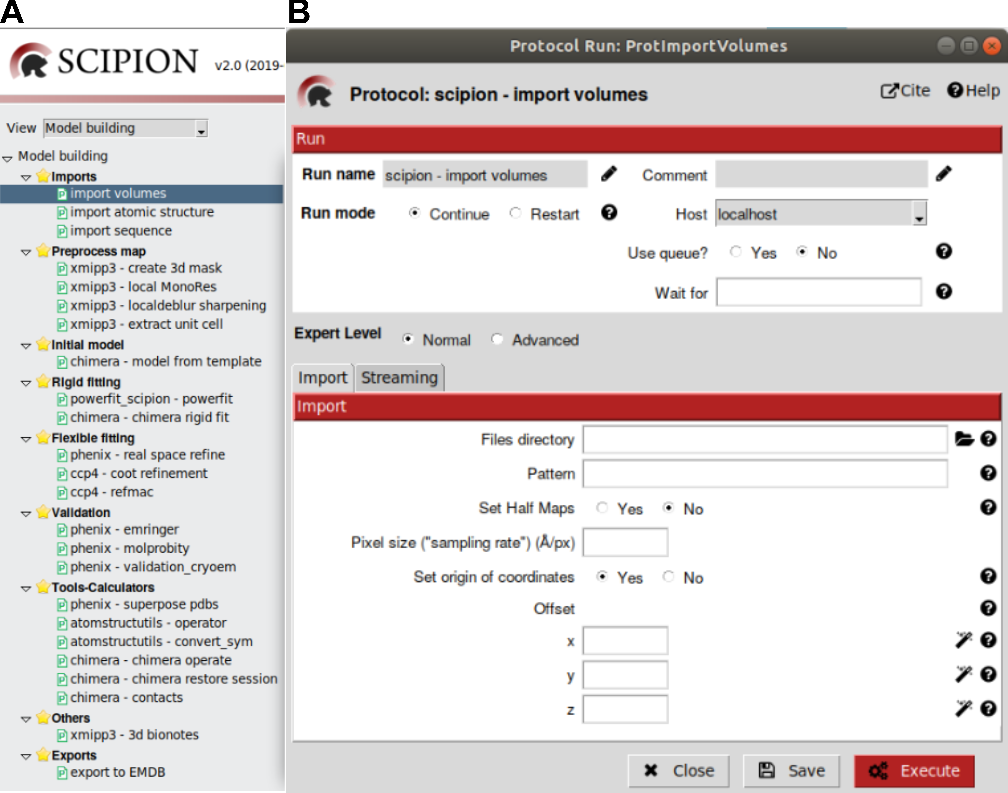
\includegraphics[width=0.90\textwidth]{Images_appendix/Fig100.pdf}
    \caption{Protocol \scommand{import volumes}. A: Protocol location in \scipion menu. B: Protocol form.}
    \label{fig:app_protocol_volume_1}
   \end{figure}
  
  \begin{itemize}
   \item \ttt{Input} section\\
  

  \begin{itemize}
   \item \ttt{Files directory}: Folder that contain one or several volumes (a set of volumes) that you'd like to import. By clicking the folder symbol right to the \ttt{Files directory} box, a browser will be opened to allow you look for the volume(s)-containing file in your computer. Click the volume that you want to select, if only one volume is going to be loaded. If a set of volumes from the same folder are going to be loaded, click the respective folder.\\
   \item \ttt{Pattern}: In case you'd like to import a set of volumes, you can include here the common name pattern to all of them. Read the help section (question mark) of this parameter and the previous parameter \ttt{Files directory} to know about wildcard characters that can be used to generalize patterns.\\
   \item \ttt{Copy files?}: Advanced parameter set to ``No'' by default because copy density maps unnecessarily duplicates disk space occupied by them, space that could be quite big. Then, by default, volumes will be downloaded by a symbolic link to the file location in your computer. Set this parameter to ``Yes'' only if you plan to transfer the project to other computers in order to preserve map data in the \scipion project.\\
   \item \ttt{Pixel size (``sampling rate'')} (\AA/px): The size of building blocks (the smallest units) of images depend on the microscope camera and magnification conditions used to get the data.\\
   \item \ttt{Set origin of coordinates}: You have to choose between setting the default origin of coordinates (option ``No'') or another origin of coordinates (``Yes''). In the option by default, the center of the electron density map will be placed in the origin of coordinates. This is the preferred option in case you want to run afterwards programs that require symmetry regarding the origin of coordinates, like the extract unit cell protocol. If you decide to set your own origin of coordinates (option ``Yes''), a new form parameter (\ttt{Offset}) will appear below.\\
   \item \ttt{Offset}: Write here x, y, and z coordinates of your preference (in \AA). Suggestions for coordinates can be obtained by pressing the wizard symbol located at the right side of the \ttt{Offset} parameter. In map files with format .mrc, suggested coordinates will be read from the map header.\\
   \end{itemize}
   
  \item \ttt{Streaming} section\\
  
  Go to this section if you plan simultaneous data acquisition and processing, and select the option ``Yes''. By default, \scipion considers that you run your processes once you have finished data acquisition (option ``No'').\\
  
  \end{itemize}
  \item Protocol execution:\\
  
  Press the \ttt{Execute} red button at the form bottom.\\
  Adding specific volume label is recommended in \ttt{Run name} section, at the form top. If you want to run again this protocol, do not forget set to \ttt{Restart} the \ttt{Run mode}.\\
  
  \item Visualization of protocol results:\\
  
  After executing the protocol, press \ttt{Analyze Results} and a small window will be opened (\ffigure{fig:app_protocol_volume_2}). This window allows you to select between \ttt{chimera} ($Chimera$ graphics window) and \ttt{slices} ($ShowJ$, the default \scipion viewer), to visualize the volume.
  
  \begin{figure}[H]
    \centering 
    \captionsetup{width=.7\linewidth} 
    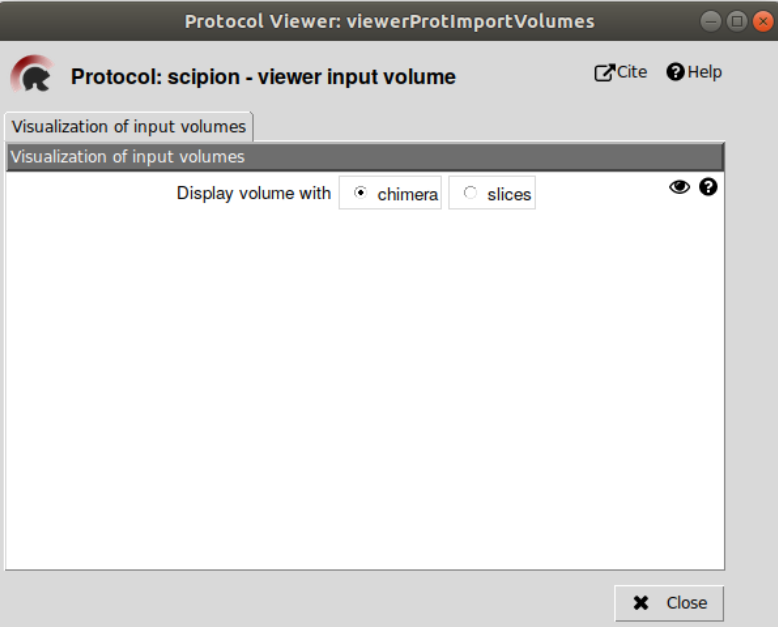
\includegraphics[width=0.90\textwidth]{Images_appendix/Fig101.pdf}
    \caption{Protocol \scommand{import volumes}. Menu to select a visualization tool.}
    \label{fig:app_protocol_volume_2}
   \end{figure}
   
   \begin{itemize}
   \item \ttt{chimera}: $Chimera$ graphics window\\
   
   Volumes in $Chimera$ are referred to the origin of coordinates. To show the relative position of the volume, the three coordinate axes are represented; x axis (red), y axis (yellow), and z axis (blue). Coordinate axes and imported volume are model numbers \#0 and \#1, respectively, in $Chimera$ \ttt{Model Panel} (\ffigure{fig:app_protocol_volume_3}). Volume coordinates and pixel size can be checked in $Chimera$ main menu \ttt{Tools -> Volume Data -> Volume Viewer -> Features -> Coordinates: Origin index/ Voxel size}. Take into account that coordinates appear in pixels while they have been introduced in \AA.
   
   \begin{figure}[H]
   \centering 
    \captionsetup{width=.7\linewidth} 
    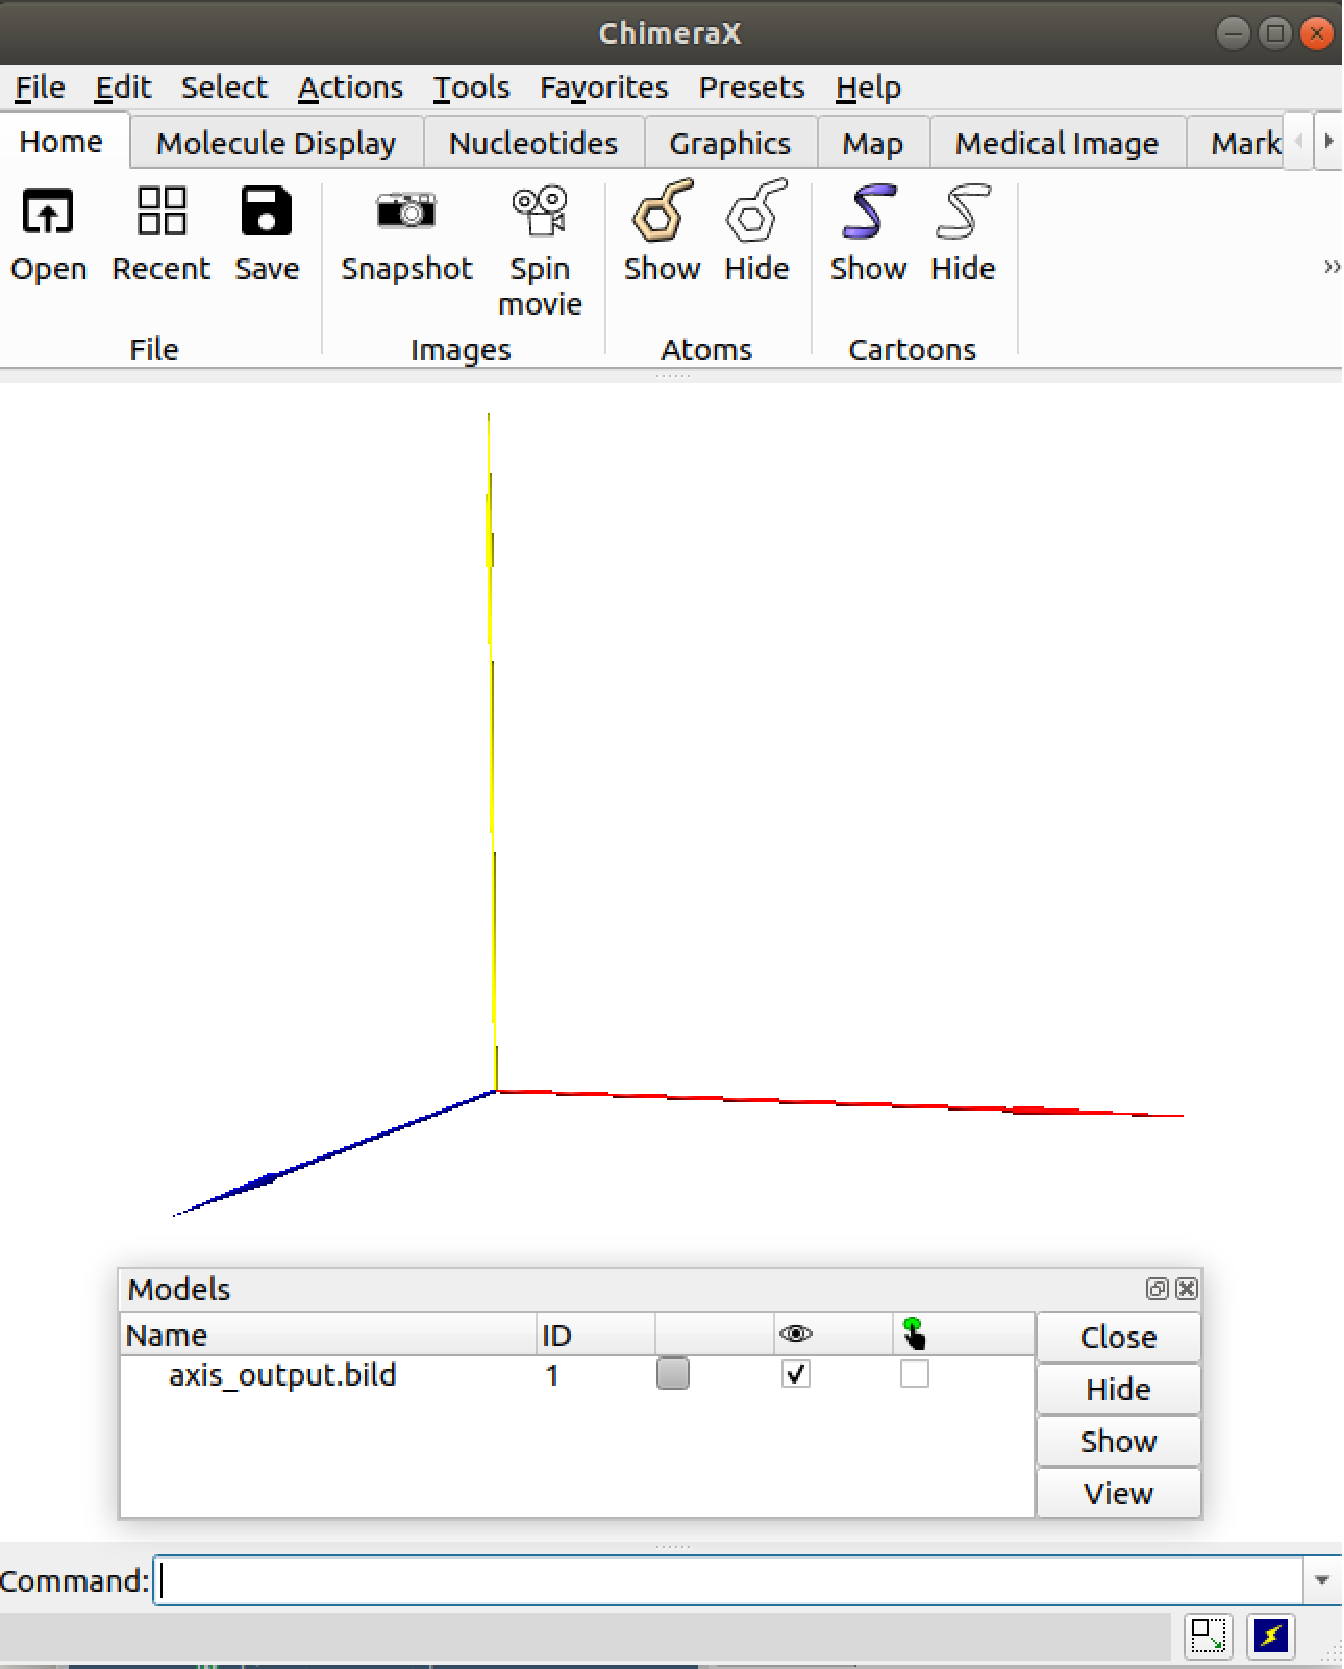
\includegraphics[width=0.90\textwidth]{Images_appendix/Fig102.pdf}
    \caption{Protocol \scommand{import volumes}. Default $Chimera$ graphics window with coordinate axes.}
    \label{fig:app_protocol_volume_3}
    \end{figure}
   
  \item \ttt{slices}: $ShowJ$\\
   
\url{https://github.com/I2PC/scipion/wiki/ShowJ}


   \begin{figure}[H]
   \centering 
    \captionsetup{width=.7\linewidth} 
    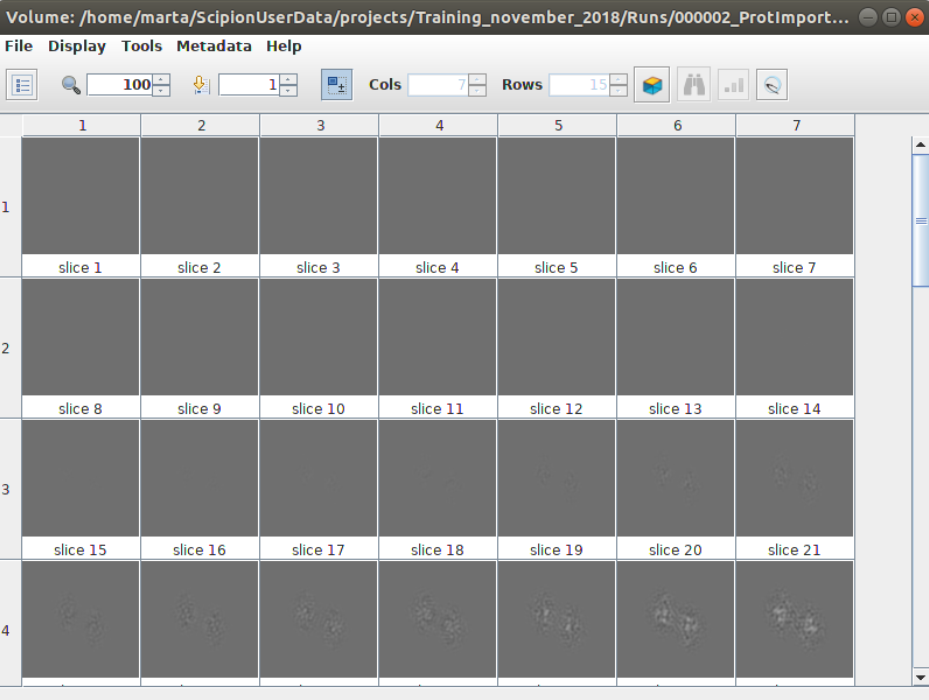
\includegraphics[width=0.90\textwidth]{Images_appendix/Fig103.pdf}
    \caption{Protocol \scommand{import volumes}. Gallery model of $ShowJ$ to visualize volume slices.}
    \label{fig:app_protocol_volume_4}
   \end{figure}
   
   \end{itemize}
   
   \item Summary content:\\
   
   Protocol output (below \scipion framework): Volume (x, y, and z dimensions, sampling rate).\\
   \ttt{SUMMARY} box:\\Path from which the volume has been downloaded.\\Sampling rate.
  
  \end{itemize}
